\section{Intermediate coupling: the transition between coupling schemes}

\begin{frame}{In theory}
    \begin{figure}
        \centering
        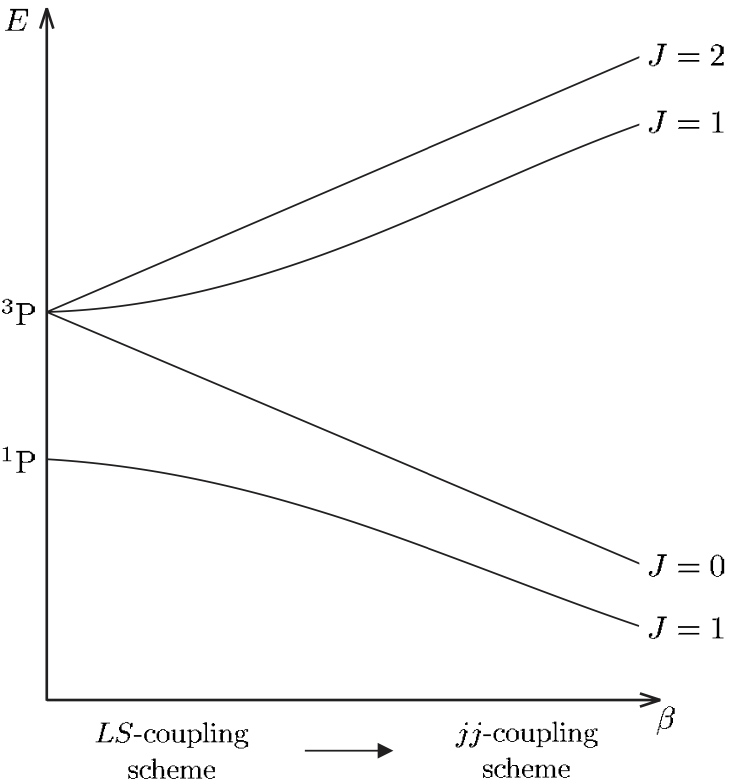
\includegraphics[scale=0.3]{fig/fig 5.10.png}
        \footnote{$\beta$: the spin–orbit interaction parameter.}
        \caption{sp configuration}
    \end{figure}
    
    As $\beta$ increases further the spin–orbit and residual electrostatic interactions become comparable and the LS-coupling scheme ceases to be a good approximation: the interval rule and (LS-coupling) selection rules break down. At large $\beta$ the jj-coupling scheme is appropriate.
\end{frame}

\begin{frame}{In theory and experiment}
    \begin{figure}
        \centering
        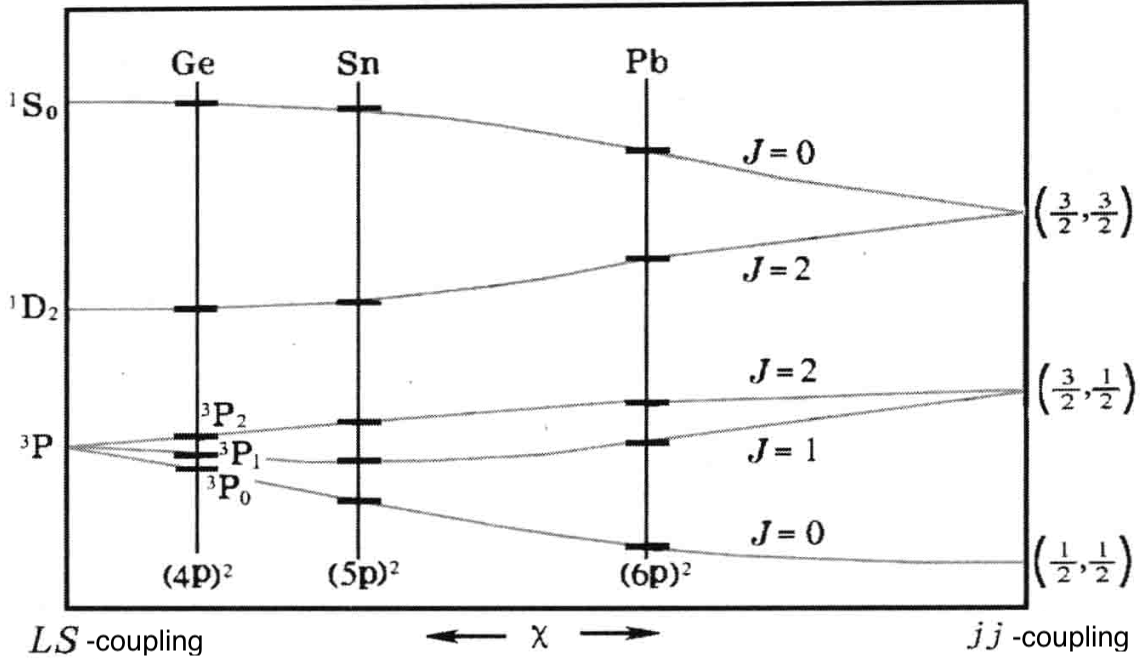
\includegraphics[scale=0.4]{fig/fig 5.11.png}
        \footnote{$\chi$: characteristic parameter.}
        \caption{$\mathrm{p}^2$ configuration}
    \end{figure}
    \centering
    A evident transition by $\chi$.
\end{frame}

\begin{frame}{In experiment}
    \begin{columns}
        \column{0.68\textwidth}
            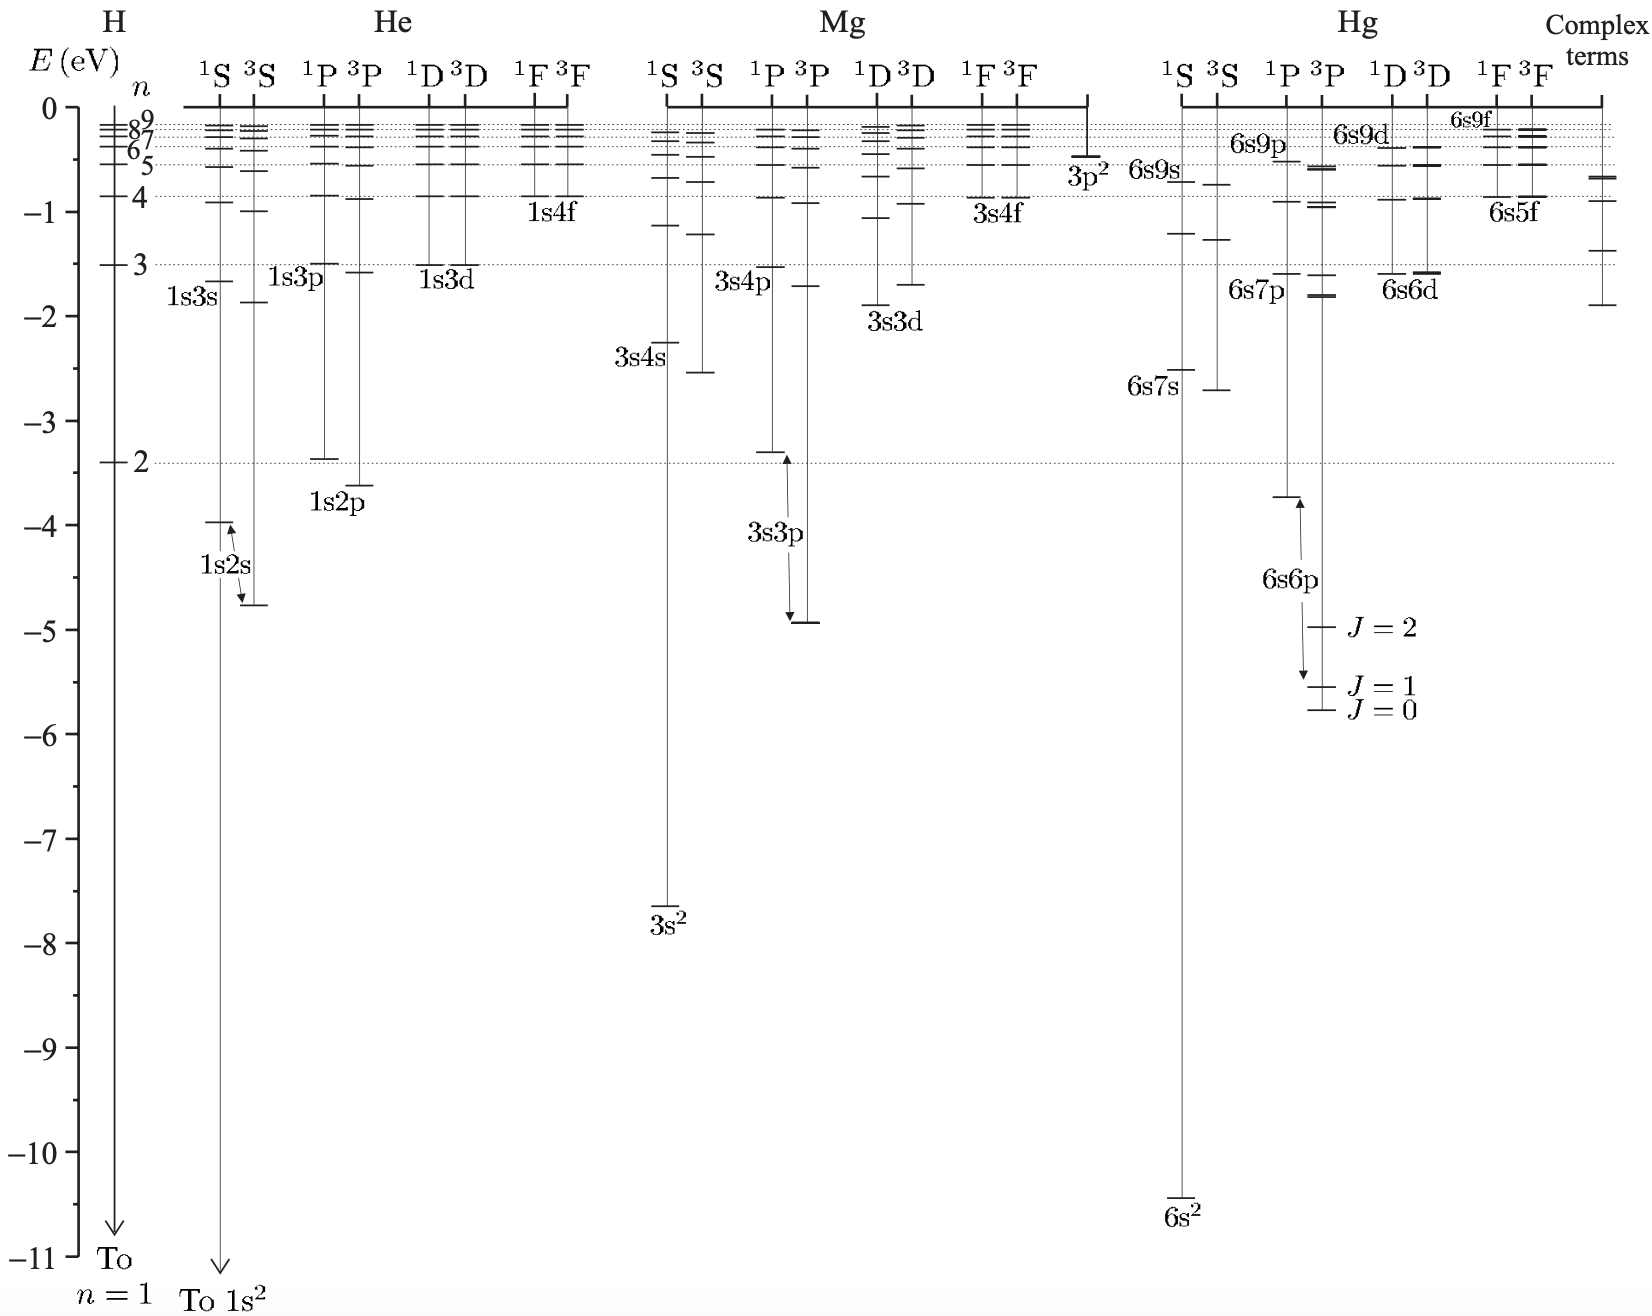
\includegraphics[scale=0.28]{fig/fig 5.12.png}
            Even for Hg, the LS-coupling scheme gives a closer approximation than the jj-coupling scheme.
    \only<2>{
        \column{0.36\textwidth}
            \begin{table}
                \centering
                \begin{tabular}{cc}
                    \hline
                    3s3p, Mg & 6s6p, Hg \\
                    \hline
                    2.1850 & 3.76 \\
                    2.1870 & 3.94 \\
                    2.1911 & 4.40 \\
                    3.5051 & 5.40 \\
                    \hline
                \end{tabular}
                \caption{$E$/\unit{m^{-1}}}
            \end{table}
            e.g. for the 6s6p configuration the $E_{\mathrm{re}}>E_{\mathrm{s-o}}$ but the interval rule is not obeyed because the spin-orbit interaction is not very small compared to the residual electrostatic interaction.}
    \only<3>{
        \column{0.36\textwidth}
            \begin{table}[]
                \centering
                \begin{tabular}{c|c}
                    \hline
                    $J$ & $E$ (\unit{m^{-1}}) \\
                    \hline
                    2 & 16908687 \\
                    1 & 16908694 \\
                    0 & 16908793 \\
                    1 & 17113500 \\
                    \hline
                \end{tabular}
                \caption{The 1s2p configuration in helium}
            \end{table}
            The interval rule is not obeyed: This occurs in helium because spin–spin and spin–other-orbit interactions have an energy comparable with that of the spin–orbit interaction.}
    \end{columns}
\end{frame}